%%%%%%%%%%%%%%%%%% ATLAS

\section{The ATLAS experiment}
\label{sed:cern:atlas}

\gls{atlas} \cite{atlas:atlas}, shown in Figure \ref{fig:atlas:atlas}, is the largest of the \gls{lhc} detectors, 
measuring 44 meters in length and 25 meters in height, and weighting about 700 tons. 
To be fully functional in the \gls{lhc} environment,  the \gls{atlas} detector needs to be fast in order to resolve the collisions resulting from consecutive bunches (which are interspaced by 25 ns) and radiation resistant. 

\begin{figure}[ht]
\centering
\subfigure{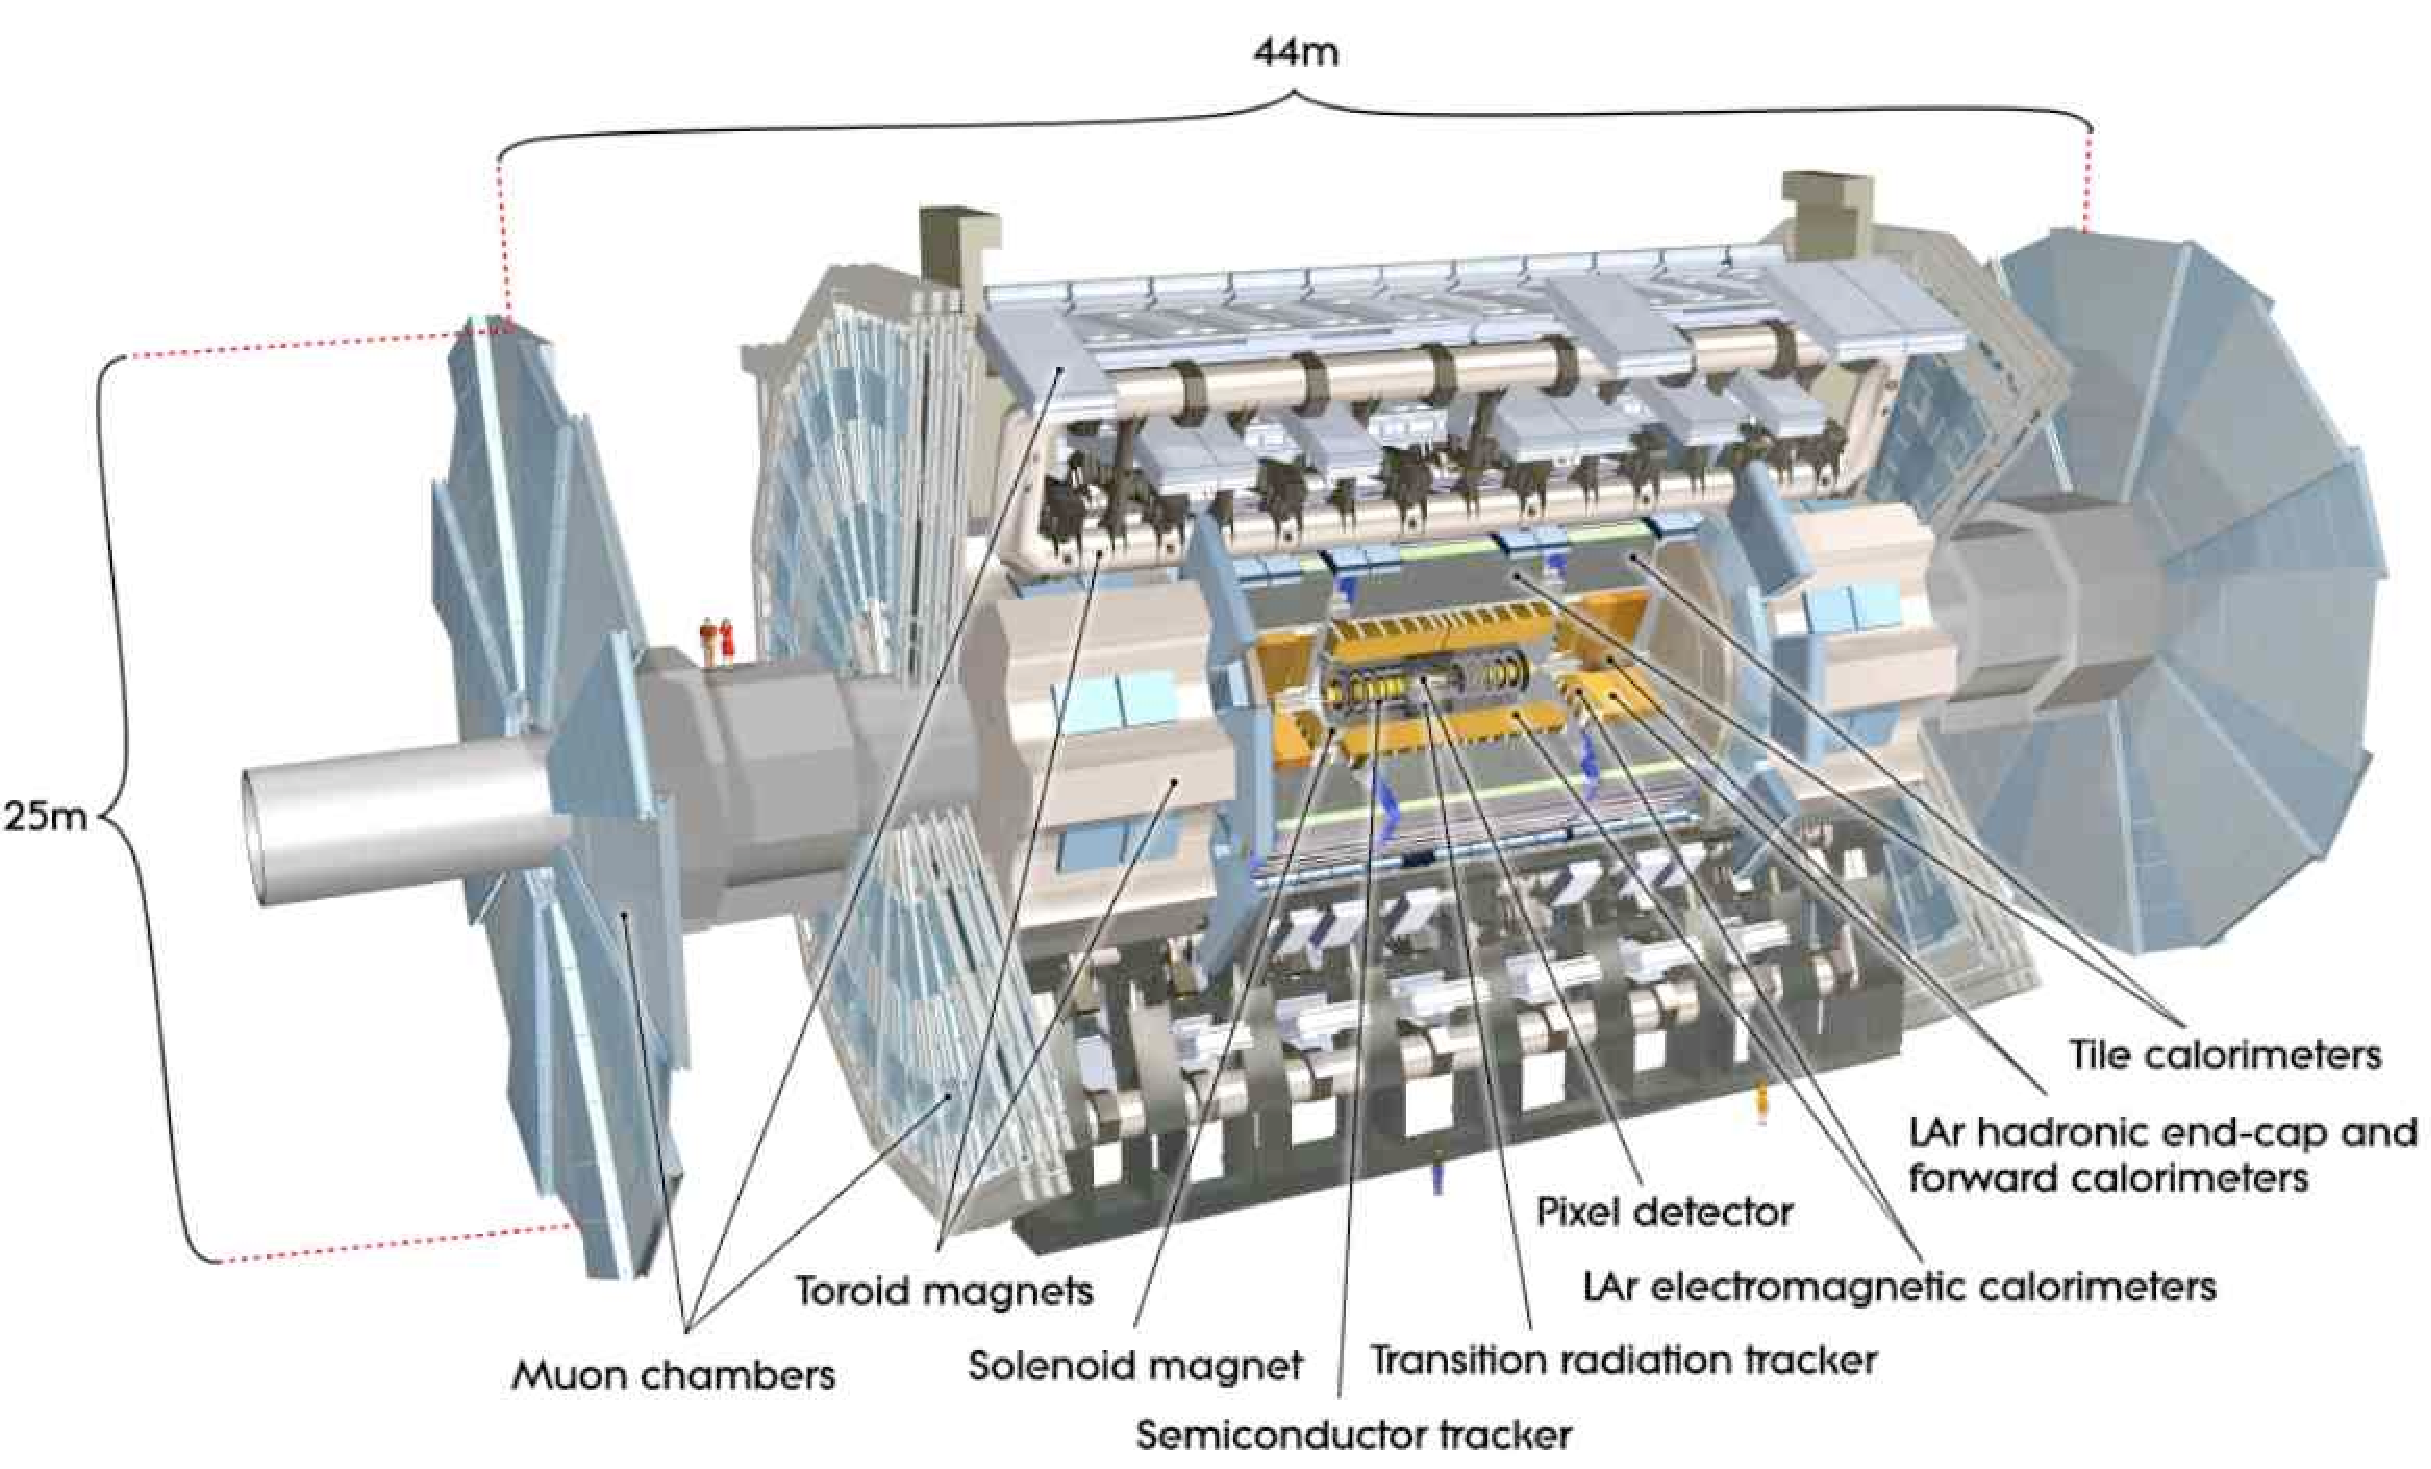
\includegraphics[width=0.85\textwidth]{figures/atlas/atlas}}
\caption{Drawing of the \gls{atlas} detector showing the different subdetectors and
the magnet systems. Figure from Ref. \cite{atlas:atlas}.}
\label{fig:atlas:atlas}
\end{figure}

The \gls{atlas} physics program covers a large variety of topics: 
\begin{itemize}
\item \textit{Standard Model} processes can be measured at the \gls{lhc} at energies never reached before, and being sensitive to them is essential both to provide accurate measurements and to use them as candles to calibrate the detector. 
\item The discovery of the \textit{Higgs boson} was one of the main goals of the \gls{lhc} and, after its observation in 2012, the focus moved onto measuring its properties. 
\item Compared to the Tevatron, the \gls{lhc} is a true \textit{top-quark} factory, 
and the study of the properties of this particle can both probe the \gls{sm} and set limits on \gls{bsm} theories.
\item The \gls{lhc} offers an exciting opportunity to discover \textit{\gls{bsm} physics}, and \gls{atlas} needs to be ready to identify its signs.
\item Despite the ALICE detector is specifically designed to study heavy-ion collisions, \gls{atlas} also carries out a \textit{heavy-ion program}.
\end{itemize}

To cope with the wide range of types and energies (from few GeV to several TeV) of particles that need to be identified, \gls{atlas} relies on a sequence of subdetectors nested in a cylindrical geometry, that follow the general schema discussed in Section \ref{sec:detectors:identification}: close to the \gls{ip} we find the \gls{id}, embedded in a solenoidal magnetic field of 2 T. The following layers are the \gls{ecal} and \gls{hcal}, and the outermost part is occupied by the muon system, where muons are bent by a 4 T toroidal magnetic field. All these components are described in the next sections.

\subsection{Coordinate system}

\gls{atlas} uses a right-handed coordinate system, with its origin at the nominal \gls{ip}. The $z$-axis follows the beam direction, while in the transverse plane the $y$-axis points upward and the $x$-axis toward the \gls{lhc} center. Positive and negative values of the $z$-axis identify respectively the A-side and the C-side of the detector. When spherical coordinates are used, the \textit{azimuthal angle} $\phi$ is defined starting from the $x$-axis, and ranges between $-\pi$ and $\pi$; the \textit{polar angle} $\theta$ is defined starting from the $z$-axis and takes values between $0$ and $\pi$. Often the polar angle is substituted by the \textit{pseudorapidity}: 
 
\begin{equation}
\eta = - \ln\tan\left(\frac{\theta}{2}\right) \; ,
\label{eq:cern:eta}
\end{equation}

\noindent which, in the limit of massless particles, is equivalent to the \textit{rapidity}:

\begin{equation}
y = \frac{1}{2} \ln\left(\frac{E + p_z}{E - p_z}\right) \; ,
\label{eq:cern:y}
\end{equation}

\noindent where $E$ is the energy of the particle and $p_z$ its momentum projected on the $z$-axis. 
The advantage of rapidity and pseudorapidity over the polar angle is that rapidity differences $\Delta y$ are boostinvariant
along the $z$-axis, as well as pseudorapidity differences $\Delta \eta$ for massless particles.
The pseudorapidity is usually preferred to the rapidity as it does not require
knowing the particle’s mass but only its polar position.
The $\eta$-$\phi$ plane is used to define the angular separation of two objects in the detector:

\begin{equation}
\Delta R = \sqrt{ (\Delta \eta)^2 + (\Delta \phi)^2  } \; .
\label{eq:cern:dR}
\end{equation}

Since protons are composite particles, and the hard scattering happens between its constituents, the longitudinal momentum of the partons is unknown. It is therefore useful to define the \textit{transverse momentum} as the projection of the momentum on the ($x$,$y$) plane: 

\begin{equation}
p_T = \sqrt{p_x^2 + p_y^2} \; ,
\label{eq:cern:pt}
\end{equation}

\noindent where $p_{x(y)}$ are the projection of the momentum along the $x$-($y$-)axis.



\subsection{Magnet system}
\label{sec:atlas:magnets}

The two segments of the \gls{atlas} detector that are dedicated to tracking, the \gls{id} and the muon spectrometers, are embedded in two separate magnetic fields. A schematic overview of the \gls{atlas} magnetic system is shown in Figure \ref{fig:atlas:magnet}.
\label{sec:cern:atlasmagnets}
\begin{figure}[ht]
\centering
\subfigure{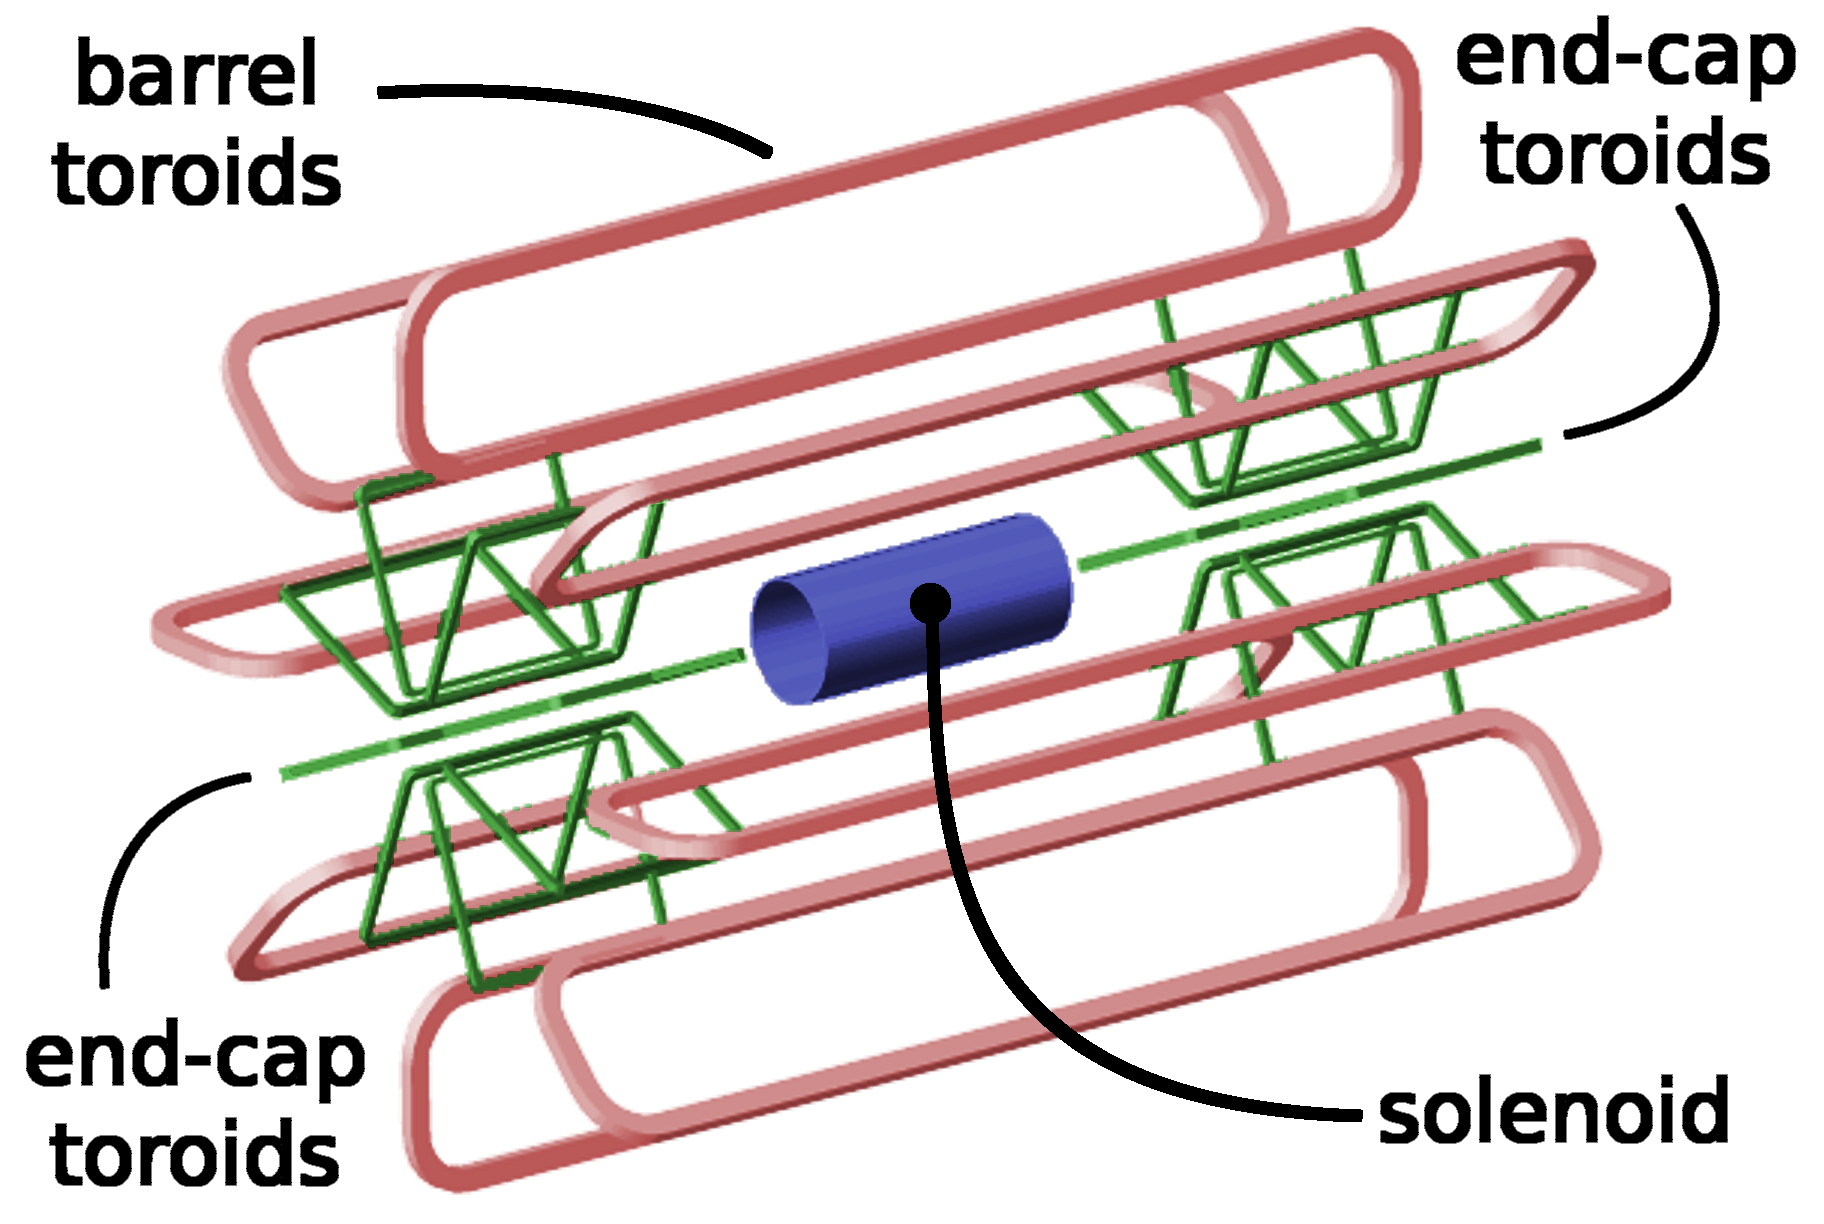
\includegraphics[width=0.45\textwidth]{figures/atlas/magnets}}
\caption{Layout of the \gls{atlas} magnet system. Figure from Ref. \cite{Goodson}.}
\label{fig:atlas:magnet}
\end{figure}

As discussed in Section \ref{sec:dec:tracking}, the magnetic field configurations that are more suitable for a detector with cylindrical symmetry are solenoidal and toroidal. The bending of the charged particles in the \gls{atlas} \gls{id} is caused by an axial 2 T solenoidal field, provided by the \textit{central solenoid} \cite{YAMAMOTO200853}. This magnet is 5.8 m long, has an inner diameter of 2.46 m and an outer diameter of 2.56. The wounded coil is made of an Al-stabilised NbTi conductor, and is powered with a 7.73 kA current. 


In the muon system, a solenoid would be disadvantageous in the measurement of forward muons, since the resultant magnetic field would not be perpendicular to the trajectory of those particles. The usage of a toroid to provide the outer magnetic field solves this problem. 
The choice of the “open air” toroid configuration allows a good muon
reconstruction performance without relying on the \gls{id}. 
The toroids allow to efficiently generate the magnetic field over a large volume with a reduced amount
of material. This minimizes the amount of multiple scattering, which represents one
of the factors limiting the muon momentum resolution.
The main drawback of the usage of a toroid is that, in order to obtain the same strength of magnetic field, a toroid needs more current than a solenoid (20.5 kA for 4 T).
The \gls{atlas} toroid system is divided into two subsystems, to allows for an easier design, 
as well as to provide access to the core part of the detector.
The \textit{barrel toroid} \cite{ATLAS:1997ac} provides a peak field of 3.9 T in the cylindrical shell between the calorimeters and the end of the muon spectrometer, and consists of eight coils contained in individual vacuum vessels.  
The \textit{end-cap toroids} \cite{ATLAS:1997ab} provide the magnetic field necessary to bend the muons in the end-cap region of the spectrometer, and each of them consists of eight coils building a single cold mass, originating a peak field of 4.1 T. 



\subsection{Inner detector}
\label{sec:atlas:id}

The main purposes of \gls{atlas} \gls{id} \cite{ATLAS:1997ag,ATLAS:1997af} are to provide a good momentum resolution of the charged particles produced in the collisions and to allow the determination of secondary vertices. The dimensions of the \gls{id} are determined on one side by the 
radius of the beam pipe and on the other side by the beginning of the \gls{ecal}. The total length is 5.4 m, which provides a coverage up to $|\eta|<$2.5.
The \gls{id} is divided into a barrel, whose schema is shown in Figure \ref{fig:atlas:id}, and two end-cap regions, covering respectively the pseudorapidity regions $|\eta|<1.2$ and $1.2<|\eta|<2.5$. In both, a mixture of gaseous and silicon detectors is used to maximize the performance and reduce the costs. The three components of the \gls{id} are the pixel detector, the semi-conductor tracker, and the transition radiation tracker, discussed in the following paragraphs.

\begin{figure}[ht]
\centering
\subfigure{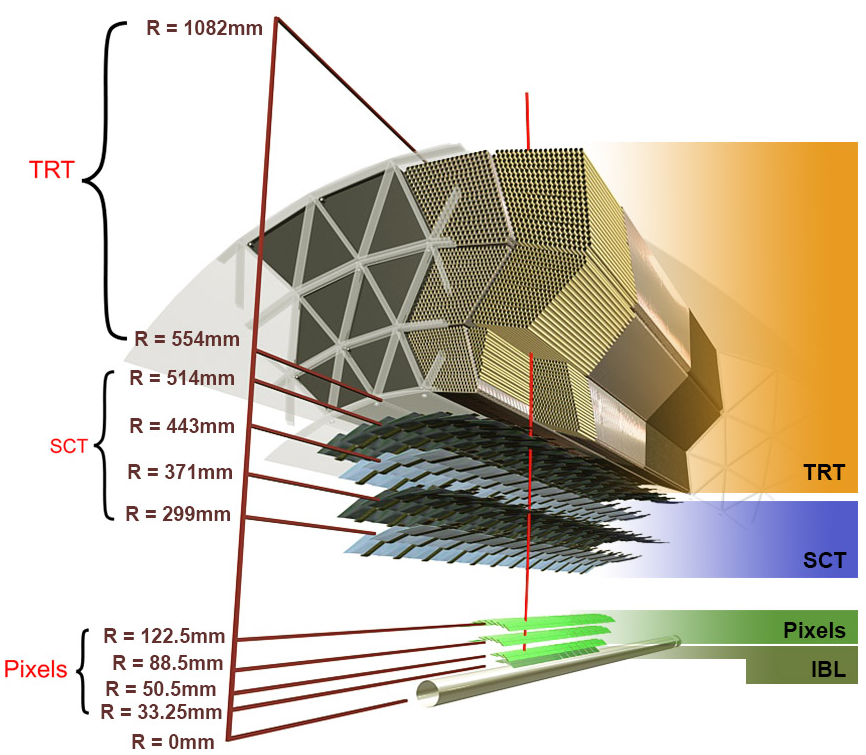
\includegraphics[width=0.65\textwidth]{figures/atlas/inner_detector}}
\caption{Layout of the \gls{atlas} \gls{id}. Figure from Ref. \cite{Potamianos:2016ptf}.}
\label{fig:atlas:id}
\end{figure}


\subsubsection*{Pixel detector}
\label{sec:atlas:pixel}
The innermost layer of the \gls{id} is the \textit{pixel detector}, divided into barrel and end-cap regions. 
During the Long Shutdown after the \gls{lhc} Run 1, the \gls{id} was subject to important upgrades \cite{Potamianos:2016ptf}. 
The main one is the addition of a fourth pixel layer in the barrel, in addition to the three already existing ones, 
the \gls{ibl} \cite{Capeans:1291633}, that is positioned 3.33 cm away from the \gls{ip}. 
In order to locate a detector so close to the \gls{ip}, the beam pipe had to be replaced with a thinner one. 
The \gls{ibl} is 72.4 cm long along the $z$-direction, and consists of 14 staves that provide full coverage in azimuthal angle. Each stave contains 20 modules, 12 with planar silicon sensors and eight with 3D pixel sensors \cite{1748-0221-7-11-P11010}, and each module has 144$\times$328 pixels with the size of 50$\times$250 $\mu$m$^2$, for a total of over 12 million pixels in the entire \gls{ibl}. The size of the pixels leads to a resolution of 40 and 8 $\mu$m respectively in the longitudinal and transverse direction. 
The three outer pixel layers are located at 5.05, 8.85 and 12.5 cm from the \gls{ip}. 
Each module contains 80 pixels of 50$\times$400 $\mu$m$^2$, leading to a spatial resolution of 115 and 10 $\mu$m respectively in the longitudinal and transverse direction. 
The two end caps, on the two sides of the detector, consist of three wheels each, with a radius of 34 cm and located at 49.5, 58.8 and 65.0 cm from the \gls{ip}. 
To ensure a good performance, the pixel detectors need to be kept at a low and stable temperature, 
between -15$^{\circ}$ C and 5$^{\circ}$ C for the \gls{ibl}, and between -15$^{\circ}$ C and -10$^{\circ}$ C for the other layers.

\subsubsection*{Semi-conductor tracker}
The \gls{atlas} \gls{sct} is composed by 4088 silicon micro-strip modules with binary readout mounted on carbon fibre composite structures, and is organized in four cylinders in the barrel and nine disks in each of the forward regions \cite{Jackson:sct}. The cylinders have  radii of 30.0, 37.3, 44.7 and 52.0 cm and provide a coverage for $|\eta|<1.1-1.4$, while the disks cover the region with $1.1-1.4<|\eta|<2.5$. 
Out of the 4088 \gls{sct} modules, 2112 modules are in the barrel, 
and contain single-sided p-in-n silicon strips, with a pitch of 80 $\mu$m. 
In each module, the strip sensors are positioned back to back with an angle of 40 mrad, to be able to access information on the $z$-coordinate as well. The end-cap modules use strips with width between 56.9 and 94.2 $\mu$m. 
These choices lead to a spatial resolution of 580 $\mu$m in the longitudinal direction and 17 $\mu$m in the transverse one.
Also the \gls{sct} components need to be kept at a low temperature, between -15$^{\circ}$ C and -5$^{\circ}$ C.

\subsubsection*{Transition radiation tracker}

The \gls{trt} is the outermost layer of the \gls{id}. In the barrel it consists of 52544 straw tubes with a length of 1.5 m disposed parallel to the beam direction, while each end-cap contains 122880 straw tubes 0.4 m long disposed perpendicularly to the beam axis. Each tube is 4 mm in diameter, and has in the inside gold plated tungsten wire as anode with a diameter of 31 $\mu$m. The tubes are filled with a mixture of 70\% Xe, 27\% CO$_2$ and 3\% O$_2$; due to a gas leakage, in 2016 part of the \gls{trt} tubes have been filled with a cheaper mixture of 80\% Ar and 20\% CO$_2$. The \gls{trt} has a pseudorapidity coverage up to $|\eta|<2$ and it provides tracking information only in the (r-$\phi$) plane, with a resolution of 130 $\mu$m.


\subsection{Calorimeters}
\label{sec:atlas:calo}

The \gls{atlas} calorimeter system is located outside the \gls{id} and the magnetic field of the solenoid, as shown in Figure \ref{fig:atlas:calo}. The \gls{ecal} is closer to the \gls{ip}, while the \gls{hcal} is on the outside; both systems have a barrel and an end-cap section. 
The combined thickness of the calorimeter system is about 11 interaction lengths to ensure the longitudinal containment of energetic jets, 
as well as a good reconstruction of the energy imbalance in the event, which is a measure of the energy carried away by neutral weakly-interacting particles. The total pseudorapidity coverage is up to $|\eta|<4.9$. 

\begin{figure}[ht]
\centering
\subfigure{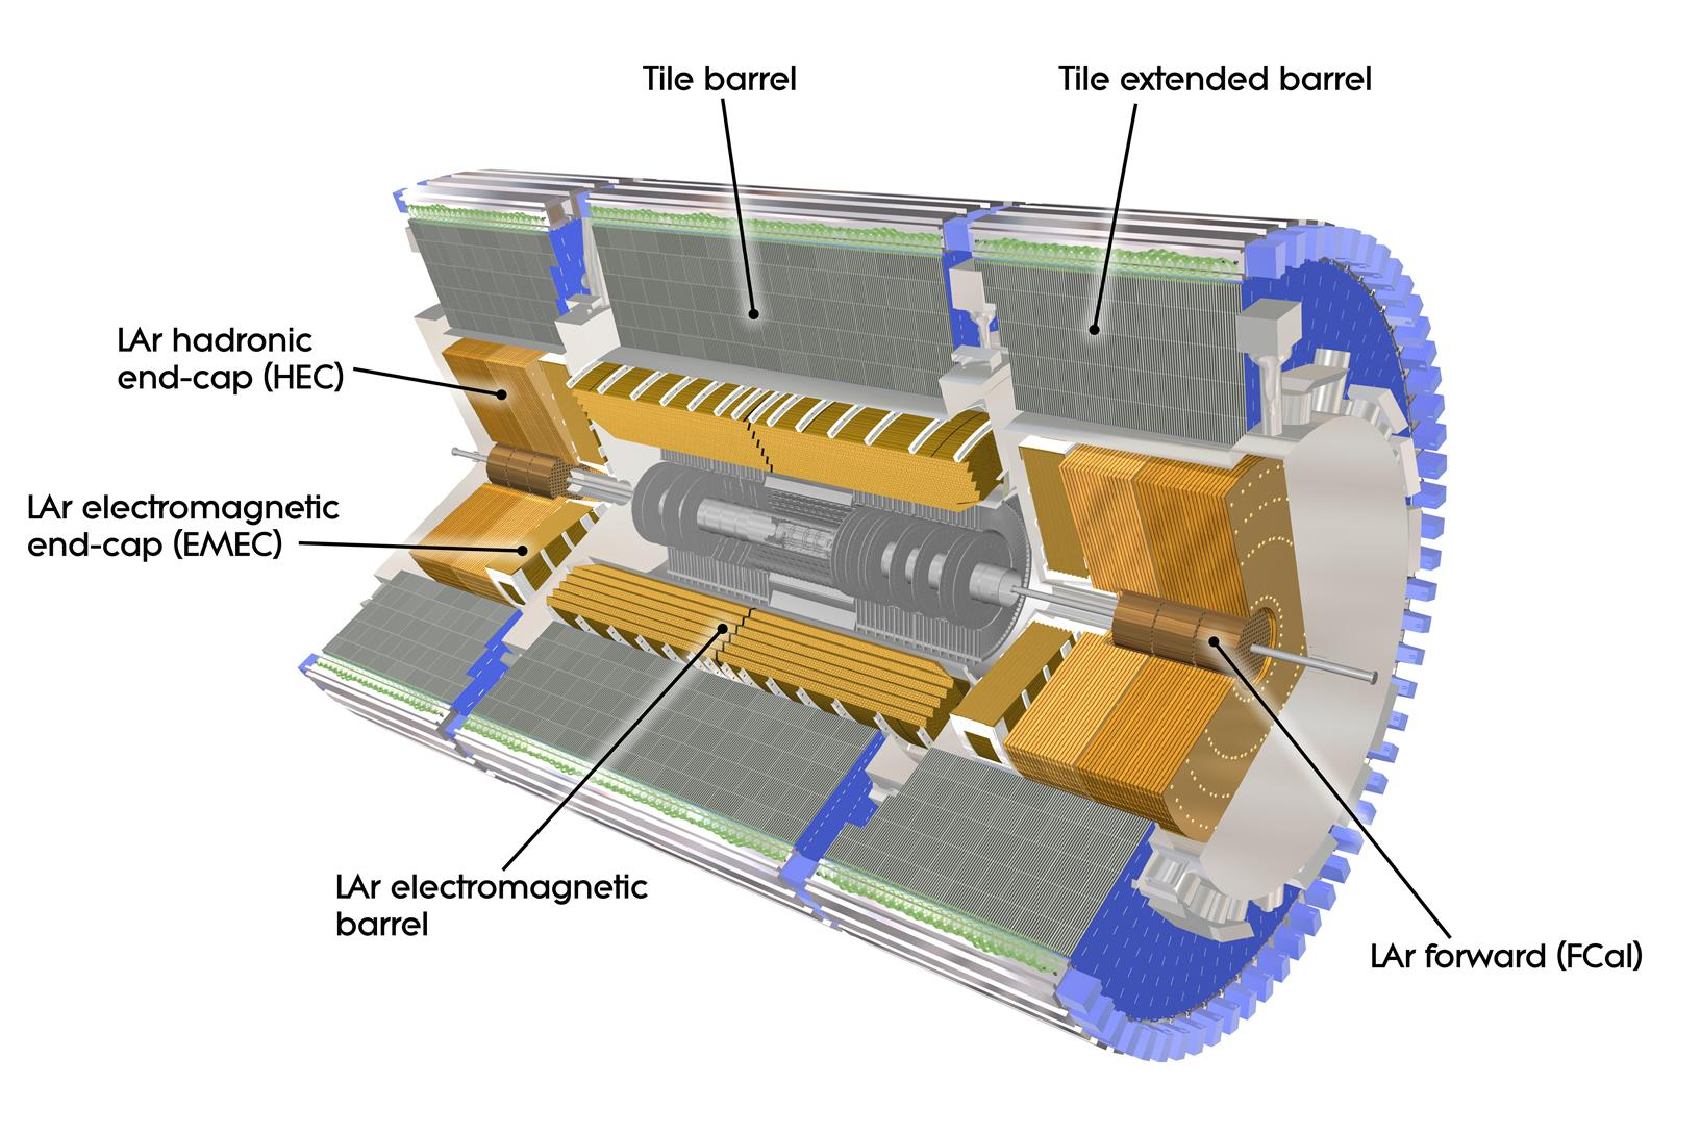
\includegraphics[width=0.75\textwidth]{figures/atlas/calorimeters}}
\caption{Layout of the \gls{atlas} calorimeter system. Figure from Ref. \cite{atlas:atlas}.}
\label{fig:atlas:calo}
\end{figure}

Table \ref{tab:atlas:cal:reso} summarizes the energy resolution of the different subsystems. As expected from the discussion in Section \ref{sec:dec:calo}, the resolution is better for electromagnetic showers than for the hadronic ones. For example, a 1 GeV particle detected in the \gls{ecal} has an energy resolution of about 19\%, while 50\% (100\%) if detected in the \gls{hcal} barrel (end-caps). On the other hand, a 1 TeV particle has an energy resolution of 0.7\% in the \gls{ecal} and 3\% (10\%) in  \gls{hcal} barrel (end-caps), and in this case the resolution is dominated by the constant term, 
related to instrumental effects and to the different response of the detectors to electromagnetic and hadronic showers. 

\begin{table}[ht]
\begin{center}
\begin{tabular}{c c }
\hline
Component & $\sigma_E / E$ \\
\hline 
\hline
\gls{ecal} & 0.1$/\sqrt{E[GeV]}$ $\bigoplus$ 0.17$/E$ $\bigoplus$ 0.007 \\ % chiara: cite LAr TDR
\hline
\gls{hcal} barrel & 0.5$/\sqrt{E[GeV]}$ $\bigoplus$ 0.03 \\
\hline
\gls{hcal} end caps & 1$/\sqrt{E[GeV]}$ $\bigoplus$ 0.1 \\
\hline
\end{tabular}
\end{center}
\caption{Energy resolution of the \gls{atlas} calorimeters.}
\label{tab:atlas:cal:reso}
\end{table}

\begin{figure}[ht]
\centering
\subfigure[]{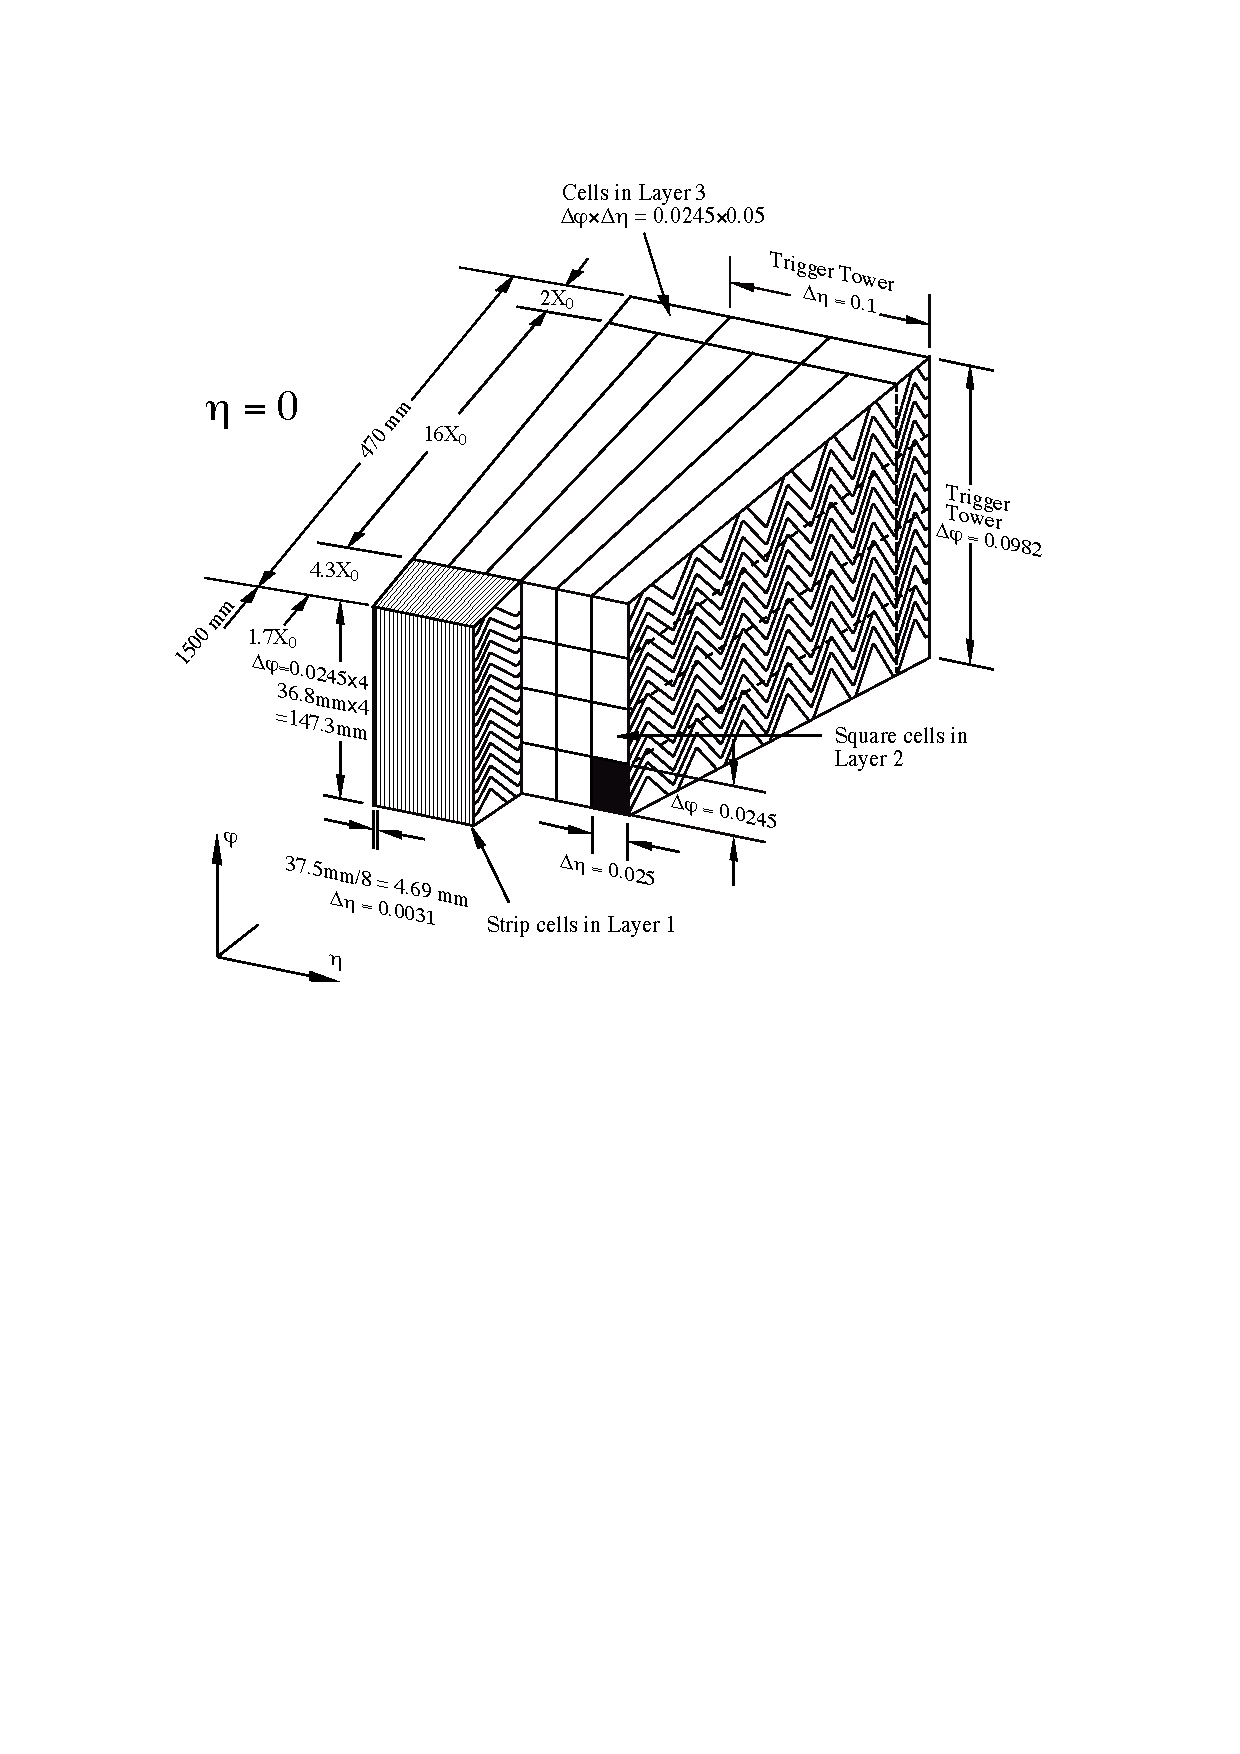
\includegraphics[width=0.495\textwidth]{figures/atlas/barrel_em.pdf}}
\subfigure[]{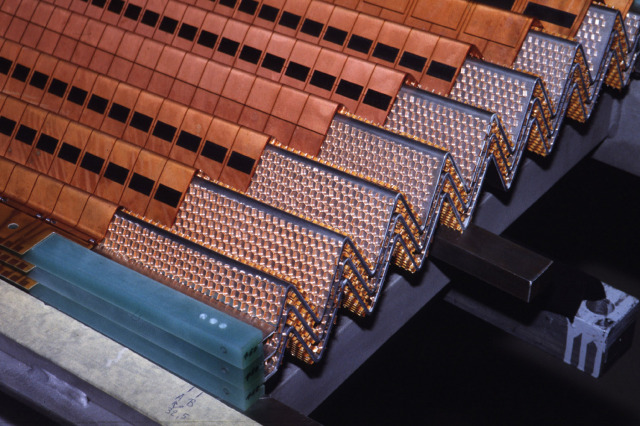
\includegraphics[width=0.495\textwidth]{figures/atlas/fisarmonica.jpeg}}
\caption{(a) Schema of a barrel module of the \gls{atlas} \gls{ecal}. Figure from Ref. \cite{atlas:atlas}. (b) Accordion shape of the metal plates of the \gls{ecal}.}
\label{fig:atlas:lar}
\end{figure}

\subsubsection*{Electromagnetic calorimeter}

The \gls{ecal} is a sampling calorimeter with \gls{lar} as active material and \textit{lead plates} as absorber, both in the barrel and in the end caps. The lead plates have a characteristic accordion shape and, in the barrel, are oriented in the radial direction. Before the \gls{ecal}, a presampler provides the information necessary to reconstruct the amount of energy lost in the passive material of the solenoid. The design of a \gls{lar} barrel module is shown in Figure \ref{fig:atlas:lar}(a), where it is possible to see the segmentation in three layers with decreasing granularity: the first layer is finely segmented in pseudorapidity, with strips of $\Delta\eta \times \Delta\phi = 0.0031 \times 0.098$; the second layer has towers of $\Delta\eta \times \Delta\phi =  0.025 \times 0.025$ to measure the clusters, while the third layer has wider towers of $\Delta\eta \times \Delta\phi =  0.05 \times 0.0245$ to provide an estimate of the energy leaking outside the \gls{ecal}. The \gls{lar} barrel offers pseudorapidity coverage up to $|\eta|<$1.475, and the thickness of the detector varies from 22 $X_0$ at $\eta=0$ to 33 $X_0$ at $|\eta|=1.3$. 
Each of the two end-cap regions consists of two coaxial wheels, of eight modules each, that cover the region $1.375<|\eta|<3.2$, with a thickness varying between 26 and 36 $X_0$ for the inner wheel and between 24 and 38 $X_0$ for the outer wheel. The end-cap modules are divided into two layers, again with decreasing granularity.


\subsubsection*{Hadronic calorimeter}

The hadronic calorimeter is composed of three subsystems with different technologies: the \gls{tilecal} \cite{TileTDR} is a sampling calorimeter with plastic scintillator as active material and steel as absorber, the \textit{hadronic end-cap calorimeter} (HEC) uses copper as absorber and liquid argon as scintillator, while the \textit{forward calorimeter} (FCal) also uses liquid argon in the active layer but has tungsten rods embedded in a copper matrix as absorber. The choice of the materials is driven by the need to have detectors more resistant to radiation in the forward region, where the flux of particles is larger. 

\gls{tilecal} covers the pseudorapidity region with $|\eta|<1.7$, and is divided into a central \gls{lb}, 5.8 m long, and two \glspl{eb}, 2.6 m long; the \gls{tilecal} inner radius is 2.28 m, and the outer radius 4.25 m. Each barrel is divided in 64 modules, disposed on the $\phi$ direction and each having the size of 0.1 radians. Each module is further segmented radially into three layers with thicknesses of about 1.5, 4.1 and 1.8 $\lambda_I$ in the \gls{lb} and 1.5, 2.6 and 3.3 $\lambda_I$ in the \gls{eb}; a schematic of one module is shown in Figure \ref{fig:atlas:tile}(a). Ionizing particles passing through the plastic scintillator (polystyrene) produce ultra-violet light, which is then collected at the two edges of each tile and converted to the longer wavelength of visible light by wavelength-shifting fibers. The fibers, with a diameter of 1 mm each, transmit the light to the readout \glspl{pmt} located in the grinder.

\begin{figure}[ht]
\centering
\subfigure[]{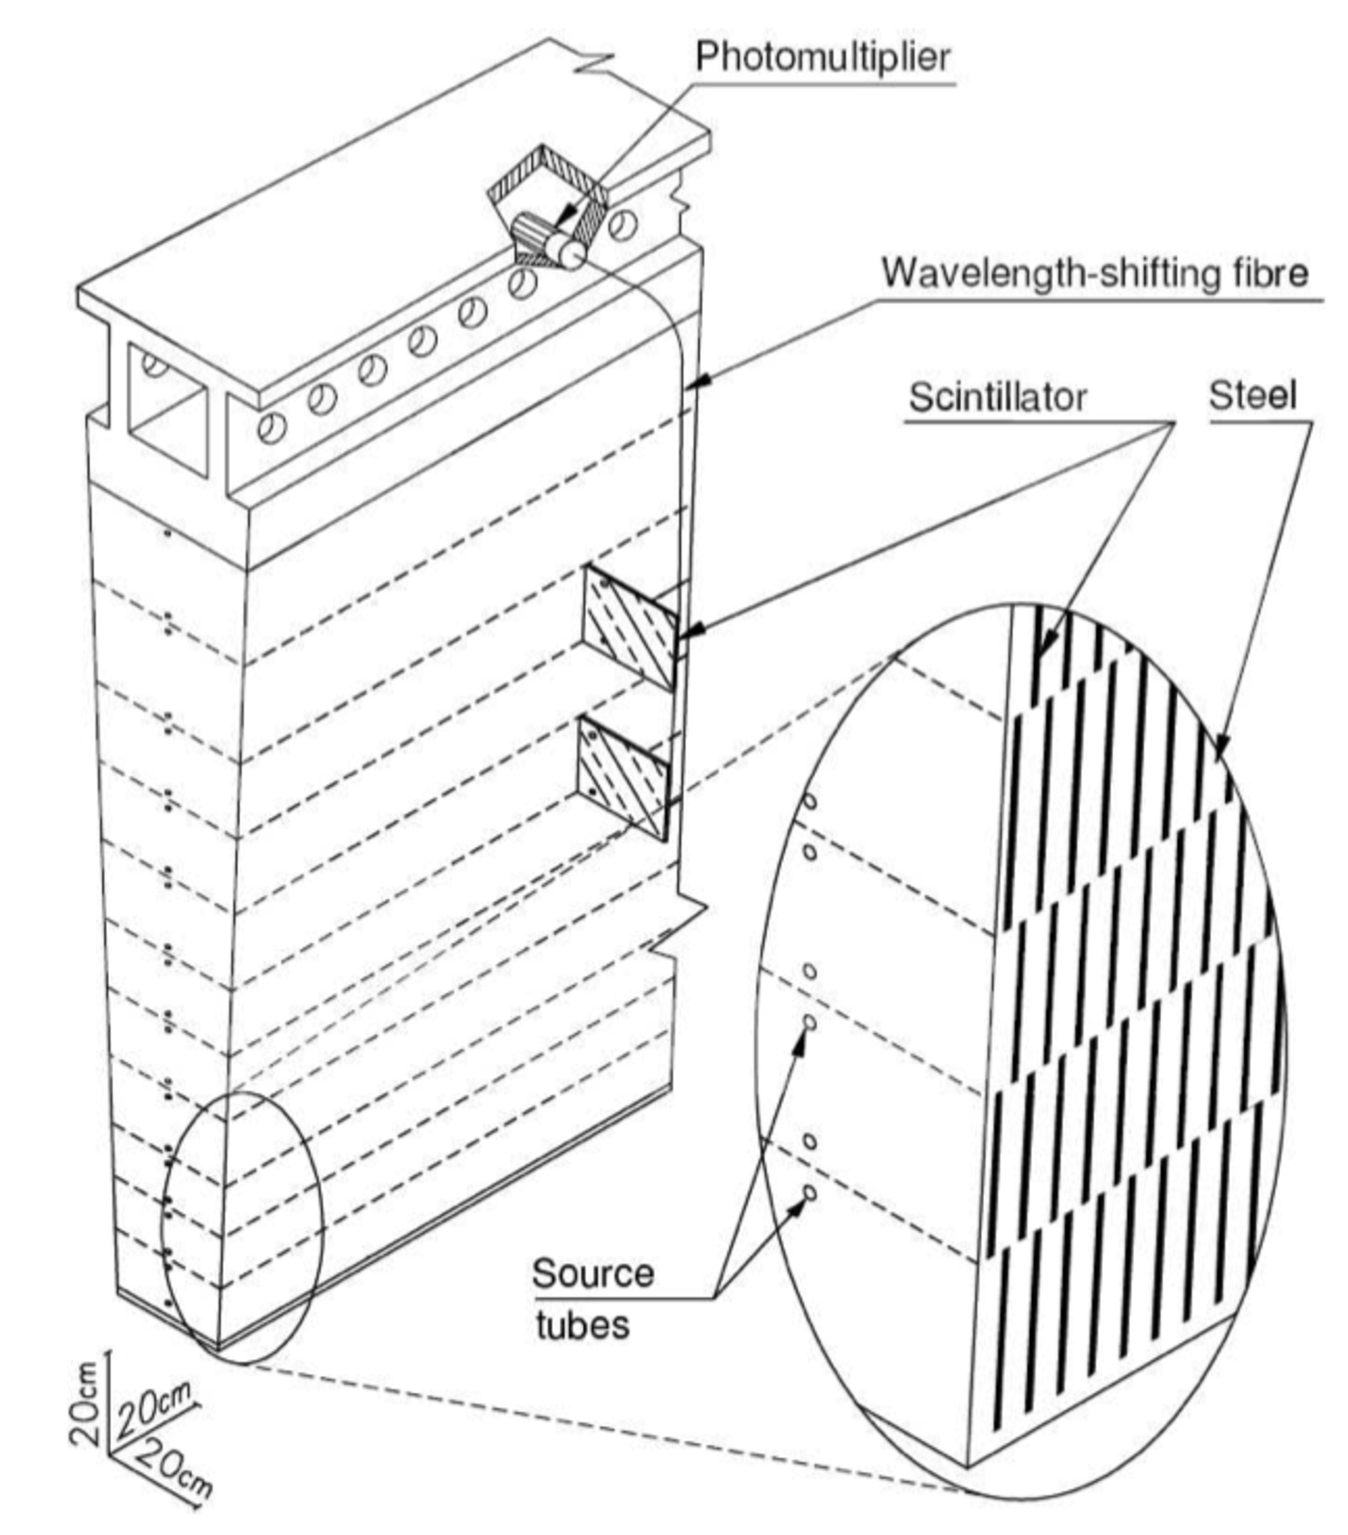
\includegraphics[width=0.4\textwidth]{figures/atlas/tile.pdf}}
\subfigure[]{\includegraphics[width=0.59\textwidth]{figures/atlas/tile_pic.pdf}}
\caption{(a) Schematic representation of a \gls{tilecal} module and its interface with the optical readout. Figure from Ref. \cite{atlas:atlas}. (b) \gls{tilecal} modules before the installation.}
\label{fig:atlas:tile}
\end{figure}

An approximately projective geometry, shown in Figure \ref{fig:atlas:tile_cells}, is provided by the grouping of the readout fibers into the \glspl{pmt}: this defines a cell structure, and each cell has dimension $\Delta\eta \times \Delta\phi = $ 0.1 $\times$ 0.1 in the first two layers and $\Delta\eta \times \Delta\phi = $ 0.2 $\times$ 0.1 in the third layer. Special cells cover the gap region between the \gls{lb} and the \gls{eb}: the gap scintillators in the pseudorapidity region $1.0<|\eta|<1.2$ and the crack scintillators in the region $1.2<|\eta|<1.6$, in front of the \gls{lar} end caps.

\begin{figure}[ht]
\centering
\subfigure{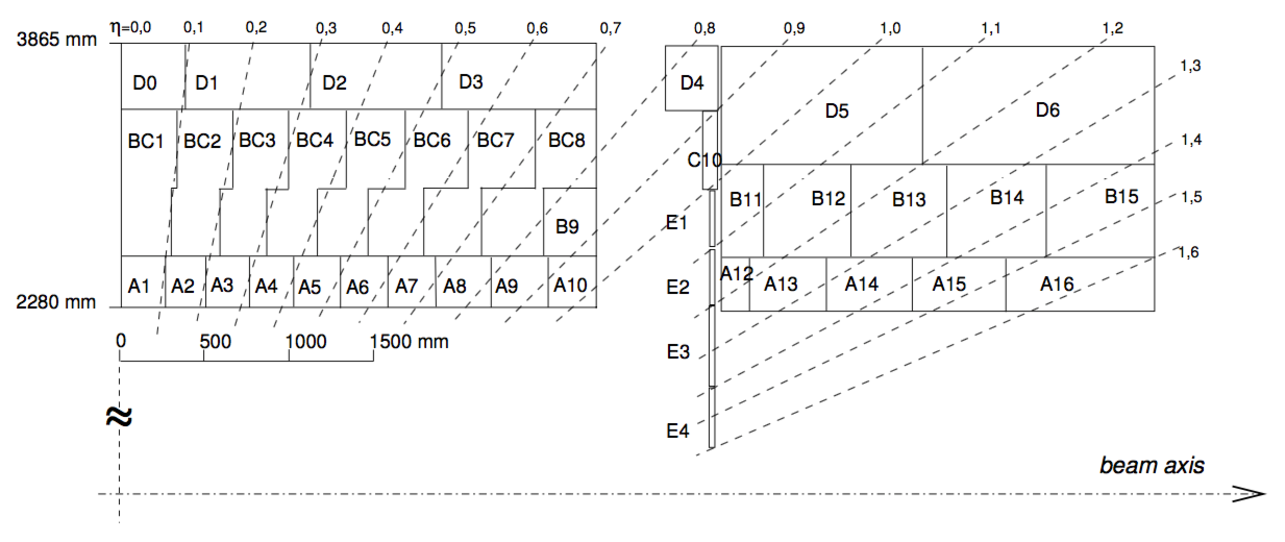
\includegraphics[width=1.0\textwidth]{figures/atlas/tile_cells.pdf}}
\caption{Layout of the projective geometry of the \gls{tilecal} cells. Figure from Ref. \cite{atlas:atlas}.}
\label{fig:atlas:tile_cells}
\end{figure}

The HEC shares the same cryogenic system as the \gls{ecal} end caps, and covers the region with $1.5<|\eta|<3.2$. Liquid argon is more resistant to radiation than the plastic scintillator used in \gls{tilecal}, and is therefore the preferred choice in the end-cap region. Each side of the HEC consists of two wheels with outer radius of 2.03 m, and each wheel is composed by 32 identical modules. The electromagnetic signal produced in the \gls{lar} is collected by cathodes on the plates. 

The FCal provides coverage in the forward region with $3.1<|\eta|<4.9$. The FCal modules are located at high pseudorapidity, at a distance of 4.7 m along the $z$-axis from the \gls{ip}.


\subsection{Muon spectrometer}

The \gls{ms} \cite{ATLAS:1997ad}, shown in Figure \ref{fig:atlas:muon}, is the outer layer of the \gls{atlas} detector, and is located in the magnetic field produced by the 4 T toroidal magnets described in Section \ref{sec:atlas:magnets}. It is designed to provide a \pt measurement with a relative uncertainty of 3\% for muons of intermediate \pt, and to maintain a low uncertainty also at higher \pt (about 10\% for muons with \pt of 1 TeV). It consists of four different muon chambers, two dedicated to the precise measurement of the muon tracks traversing the detector, 
and two providing fast event selection for the trigger system. 

\begin{figure}[ht]
\centering
\subfigure{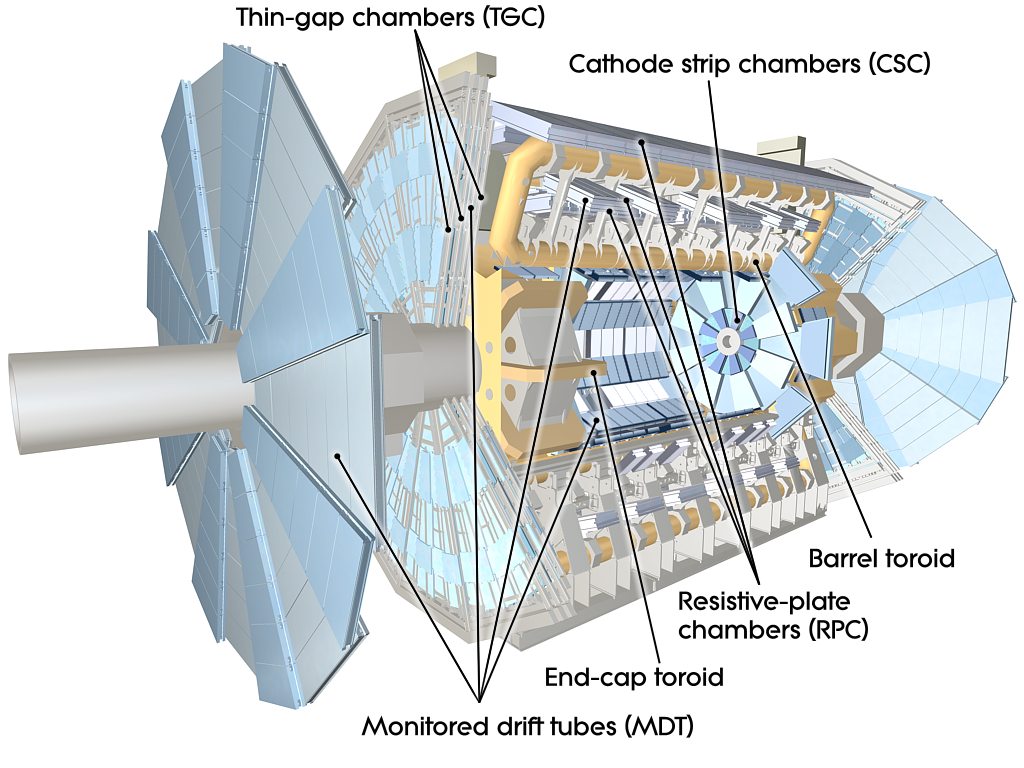
\includegraphics[width=0.65\textwidth]{figures/atlas/muon}}
\caption{Layout of the \gls{atlas} muon system. Figure from Ref. \cite{atlas:atlas}.}
\label{fig:atlas:muon}
\end{figure}

The two systems dedicated to precision measurement are the \gls{mdt} and the \gls{csc}, both present in barrel and end caps. The \glspl{mdt} are proportional drift chambers covering the region $|\eta|<2.7$; they are made of aluminium tubes with a diameter of 30 mm and a length between 700 and 6300 mm, and a cathode wire made of an alloy of tungsten (97\%) and rhenium (3\%). The filling gas is a mixture of Ar, N$_2$, and CH$_4$ with percentages respectively of 91\%, 4\% and 5\%. The \glspl{csc} are multi-wire proportional chambers that cover the region with $2.0<|\eta|<2.7$, where the shorter drift time of this detector (30 ns compared to the 480 ns of the \glspl{mdt}) allows to better cope with the increase in particle flux in the forward region. The anode wires in the \glspl{csc} are made of the same tungsten-rhenium alloy of the \glspl{mdt} and have a 2.54 mm pitch, which is the same distance separating them from the copper cathode strips, creating a symmetric cell. The gas inside the chamber is a mixture of 30\% Ar, 50\% CO$_2$, and 20\% CF$_4$. The spatial resolution is 40 $\mu$m in the bending plane and 5 mm in the perpendicular plane.

The muon trigger system needs to be able to identify events with energetic muons in a timescale compatible with assigning them to the correct bunch crossing, that are spaced by 25 ns. The two trigger chambers are the \gls{rpc} and the \gls{tgc}. The \glspl{rpc} are arranged in three layers in the barrel region, outside the outermost \gls{mdt} layer. Each narrow chamber consists of two parallel resistive bakelite plates and is filled with a mixture of 94.7\% C$_2$H$_2$F$_4$, 5\% Iso-C$_4$H$_{10}$, and 0.3\% SF$_6$. The signal is readout by metal plates through capacitive coupling, providing a time resolution of 1.5 ns, while the space resolution is about 1 cm. The \gls{rpc} also provides the $\phi$ coordinate for the track, which is not measured by the \glspl{mdt}. The \glspl{tgc} are multi-wire proportional chambers located in the end caps, filled with a mixture of 55\% CO$_2$ and 45\% n-C$_5$H$_{12}$. Contrary to the \glspl{csc}, the \glspl{tgc} are characterized by a distance between the cathode and the anode shorter than the anode pitch. The pseudorapidity coverage is $1.05<|\eta|<2.7$ for tracking and $1.05<|\eta|<2.4$ for triggering; the time response is similar to that of the \glspl{rpc}, while the spatial resolution is better: between 2 and 7 mm. 

\subsection{Luminosity measurement}
\label{sec:lumimeas}

An accurate determination of the luminosity is important both for \gls{sm} measurements, where often the luminosity uncertainty can dominate in some cases, and for \gls{bsm} searches, where a precise background estimate is a key ingredient to be sensitive to a signal. In the \gls{atlas} detector the luminosity measurement is performed with redundancy by multiple luminometers that use different technologies and algorithms, to allow a better determination of the final number and to assign systematic uncertainties. The instantaneous luminosity in Equation \ref{eq:cern:lumi} can also be expressed following the conventions in Ref. \cite{Aaboud:2016hhf} as product of the number of bunch crossings $N_b$ and the average luminosity per bunch cross $<\mathcal{L}_b>$:
\begin{equation}
\mathcal{L} = N_b <\mathcal{L}_b> = N_b \frac{f <\mu>}{\sigma_{\mathrm{inel}} } \; .
\label{eq:atlas:lumi}
\end{equation}

With respect to the nomenclature of Equation \ref{eq:cern:lumi}, $<\mu>$ is the average pileup per bunch crossing and $\sigma_{\mathrm{inel}}$ the inelastic \gls{pp} cross-section. Because of the finite acceptance and efficiency of the detector, what is measured is:
\begin{equation}
\mathcal{L}_b = \frac{f <\mu_\mathrm{vis}>}{\sigma_{\mathrm{vis}} } \; ,
\end{equation}

\noindent where $<\mu_\mathrm{vis}>$ and $\sigma_{\mathrm{vis}}$ are the product of the corresponding quantities in Equation \ref{eq:atlas:lumi} and the acceptance and efficiency of the detector. Out of these two quantities, $<\mu_\mathrm{vis}>$ is directly measurable during the collisions, while $\sigma_{\mathrm{vis}}$ is determined with the \gls{vdm} method \cite{vanderMeer:296752}, carried out in the dedicated \gls{vdm} runs. These are special runs with low bunch intensity and number of bunches, where a variation (scan) of the overlap of the two beams in the $x$- and $y$-direction is performed; the beam parameters and the peak of visible interaction rate per bunch crossing during the scan can be used to determine the visible cross-section and therefore calibrate each subsystem. 

We can express the luminosity per bunch cross as:
\begin{equation}
\mathcal{L}_b = n_1 n_2 f \int \rho_1(x,y) \rho_2(x,y) \, dx \, dy \; ,
\label{eq:lumi_vdm1}
\end{equation}

\noindent where $\rho_1(x,y)$ and $\rho_2(x,y)$ are the particle densities in the two colliding bunches at the \gls{ip}. 
Under the assumption that these densities can be factorized into the horizontal and vertical components, we can write Equation \ref{eq:lumi_vdm1} as:
\begin{equation}
\mathcal{L}_b = n_1 n_2 f  \Omega_x(\rho_1(x), \rho_2(x)) \Omega_y(\rho_1(y), \rho_2(y))  \; ,
\label{eq:lumi_vdm1}
\end{equation}

\noindent where $\Omega_{x/y}$ defines the beam overlap in the $x$/$y$ direction.

The relevant quantity in physics analyses is the integrated luminosity over a defined period of time. The basic time unit over which the integrated luminosity is computed and stored is the \gls{lub}, whose duration is defined by the \gls{atlas} trigger system and is typically about one minute. The data contained in each \gls{lub} is collected with the same detector conditions, and the integrated luminosity is computed as the average instantaneous luminosity multiplied by the \gls{lub} time duration.

\gls{atlas} has two primary specifically-designed luminometers, LUCID-2 (\textit{LUminosity measurements using Cherenkov Integrating Detector}) and BCM (\textit{Beam Conditions Monitor}), whose results are compared with the one obtained by other \gls{atlas} subsystems that measure luminosity through quantities that are sensitive to it, such as the number of tracks or the flow of particles.

\subsubsection*{Bunch-by-bunch luminometers}

The two dedicated luminometers are able to provide information for individual bunch crossings, each labeled by a \gls{bcid}.

BCM consists of four $8 \times 8$ mm$^2$ diamond sensors, located at $z= \pm 184$ m from the \gls{ip} and disposed in a cross shape around the beam pipe, at $|\eta| = 4.2$. Beside luminosity measurements, BCM is also used to recognize beam losses so that the beam can be dumped before damaging the silicon detectors. 

LUCID is located 17 m from the \gls{ip}, at $5.6 < |\eta| < 6.0$, and consists on each side of 16 Cherenkov detectors built by aluminum tubes with a diameter of 10 mm. Cherenkov radiation is produced in the passage of particles through the quartz windows of the \glspl{pmt}. A signal over threshold produces a hit for that bunch crossing.

%\begin{figure}[ht]
%\centering
%\subfigure{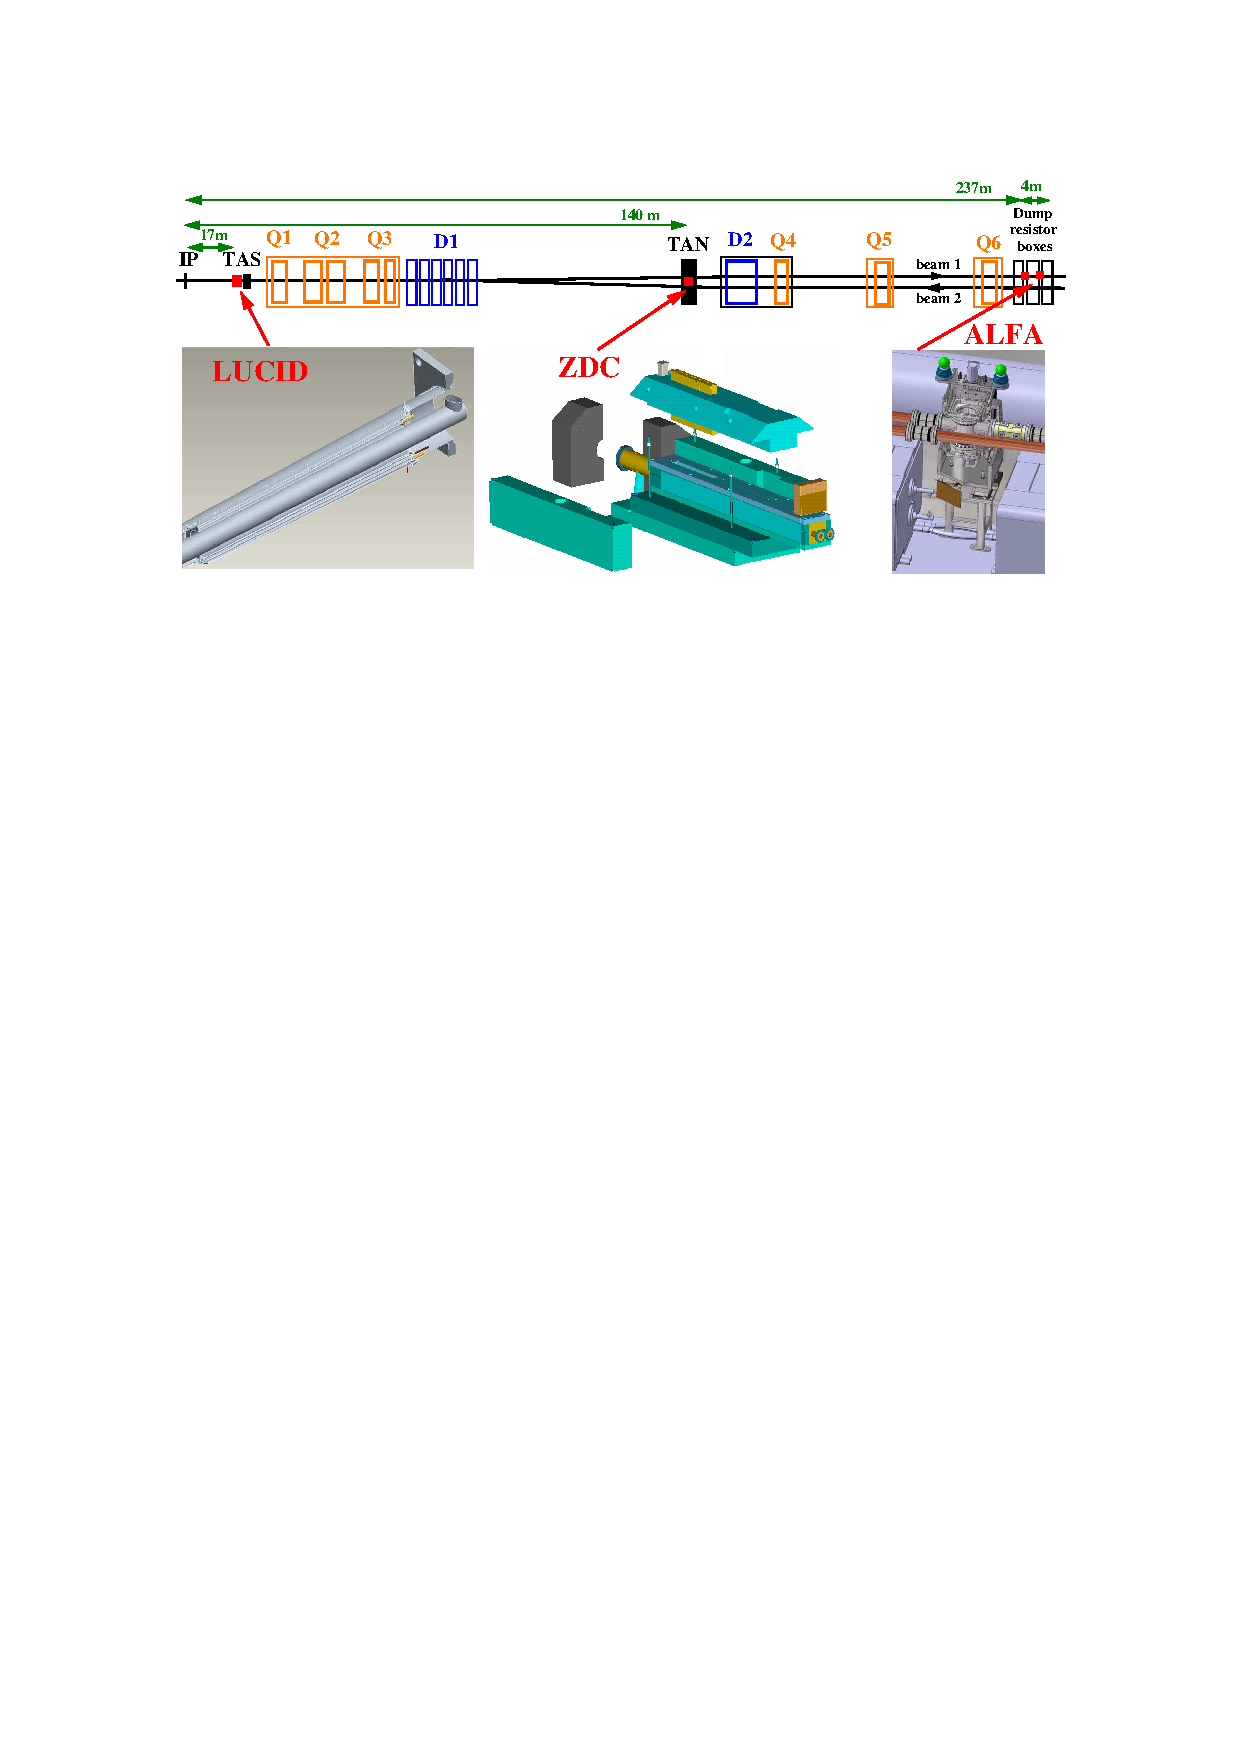
\includegraphics[width=0.75\textwidth]{figures/atlas/forward}}
%\caption{Forward detectors in \gls{atlas}.}
%\label{fig:atlas:forward}
%\end{figure}

\subsubsection*{Tracker-based algorithms}

The \gls{id}, described in Sec. \ref{sec:atlas:id}, records the passage of charged particles as tracks. The number of such charged tracks in each bunch crossing is proportional to the luminosity, and can be used as $<\mu_\mathrm{vis}>$ if averaged over a \gls{lub}. 
During collisions partial data, selected with a random trigger that has the same probability of firing for each colliding bunch, are recorded in a dedicated stream. Because of the high number of colliding bunches, to achieve enough statistical precision the luminosity is provided as integrated over the \gls{lub}; instead, during \gls{vdm} scans, bunch-by-bunch luminosity can be provided. 
% chiara: indicate which track types have been used in 2015-2016 and which in 2017
The reconstruction of the tracks used in this process is described in Sec. \ref{sec:reco:tracks}.

\subsubsection*{Bunch-integrating devices}

The long-term stability of the luminosity measurement provided by BCM, LUCID and the track system is checked with devices that are sensitive to the flux of particles through the detector. This technique only allows to measure the instantaneous luminosity integrated over a time of a few seconds, and not bunch-by-bunch.

A subdetector capable of providing such measurement is \gls{tilecal}, described in Sec. \ref{sec:atlas:calo}. The current generated by the \glspl{pmt} is proportional to the total number of particles; this current is not read through the digital readout system, but through an integrator system sensitive to currents between 0.01 nA and 1.2 $\mu$A over a time window of 10-20 ms. The current induced in different cells varies largely with the cell position: the ones that receive a larger amount of particles are the ones around $|\eta|=1.25$ and in the inner part of the detector (as the hadronic shower is stopped while it passes through the calorimeter). The \gls{tilecal} luminosity measurement is not calibrated during \gls{vdm} scans, but is instead equalized to LUCID or the track measurement for one specific run, and the calibration constant between current and luminosity allows to measure the luminosity also in different runs. More details on the \gls{tilecal} luminosity measurement are given in 
Appendix \ref{app:pmt}. 

Additional systems used in the luminosity determination are the \gls{lar}-based calorimeters in the end caps, the electromagnetic one and the FCal. In both systems the high-voltage (HV) system maintains a constant voltage by supplying a continuous injection of current that counterbalances the voltage drop caused by the flux of particles in a certain sector. The measurement of this current provides a luminosity measurement. Also \gls{lar} systems are not calibrated during the \gls{vdm} scan, but each HV run is calibrated to the baseline luminosity algorithm over a physics run.  


\subsection{Trigger system}
\label{sec:cern:trigger}

With the nominal bunch spacing of 25 ns, the \gls{lhc} produces collisions at a frequency of 40 MHz. This exceeds by several orders of magnitude the current capability to write events to disk; therefore the \gls{atlas} \gls{tdaq} system selects and records the events that are considered interesting for analyses. The \gls{tdaq} system has been updated between Run 1 and Run 2 \cite{Aaboud:2016leb} and it currently consists of a  hardware \gls{lone} trigger and a single software-based \gls{hlt}. A schematic view of the Run 2 \gls{atlas} \gls{tdaq} system is shown in Figure \ref{fig:atlas:trig}. \gls{lone} is the first step in the chain, and reduces the output rate from 40 MHz to about 100 kHz. It uses reduced-granularity information from the calorimeter systems and from the muon \gls{rpc} and TGS to select events with interesting objects and saves the information about the \gls{roi}. \gls{lone} has a latency time of 2.5 $\mu$s; this corresponds to about 100 collisions, whose information has to be temporarily stored in buffers before the \gls{lone} \gls{ctp} finalizes a decision based on the inputs from the \gls{lonecalo}, \gls{lonemuo} and the \gls{lonetopo}. 

During Run 1 the \gls{hlt} consisted of two separate levels that in Run 2 have been merged to have a simpler setup and better resource sharing. The \gls{hlt} uses information with finer granularity from the calorimeter systems, precision tracking from the muon spectrometer and tracking information from the \gls{id}, not available for \gls{lone}. The \gls{hlt} reduces further the event rate to about 1 kHz, and has a processing time of about 0.2 s per each event. 

A \textit{trigger chain} is a set of selections that characterize a certain trigger object, and the list of all available trigger chains defines the \textit{trigger menu}; some of the items on the menu are \textit{unprescaled}, which means all the events firing that trigger are stored, while others are associated to a \textit{prescale constant} P such that only a fraction $\frac{1}{P}$ of the events firing the trigger are stored.

\begin{figure}[ht]
\centering
\subfigure[]{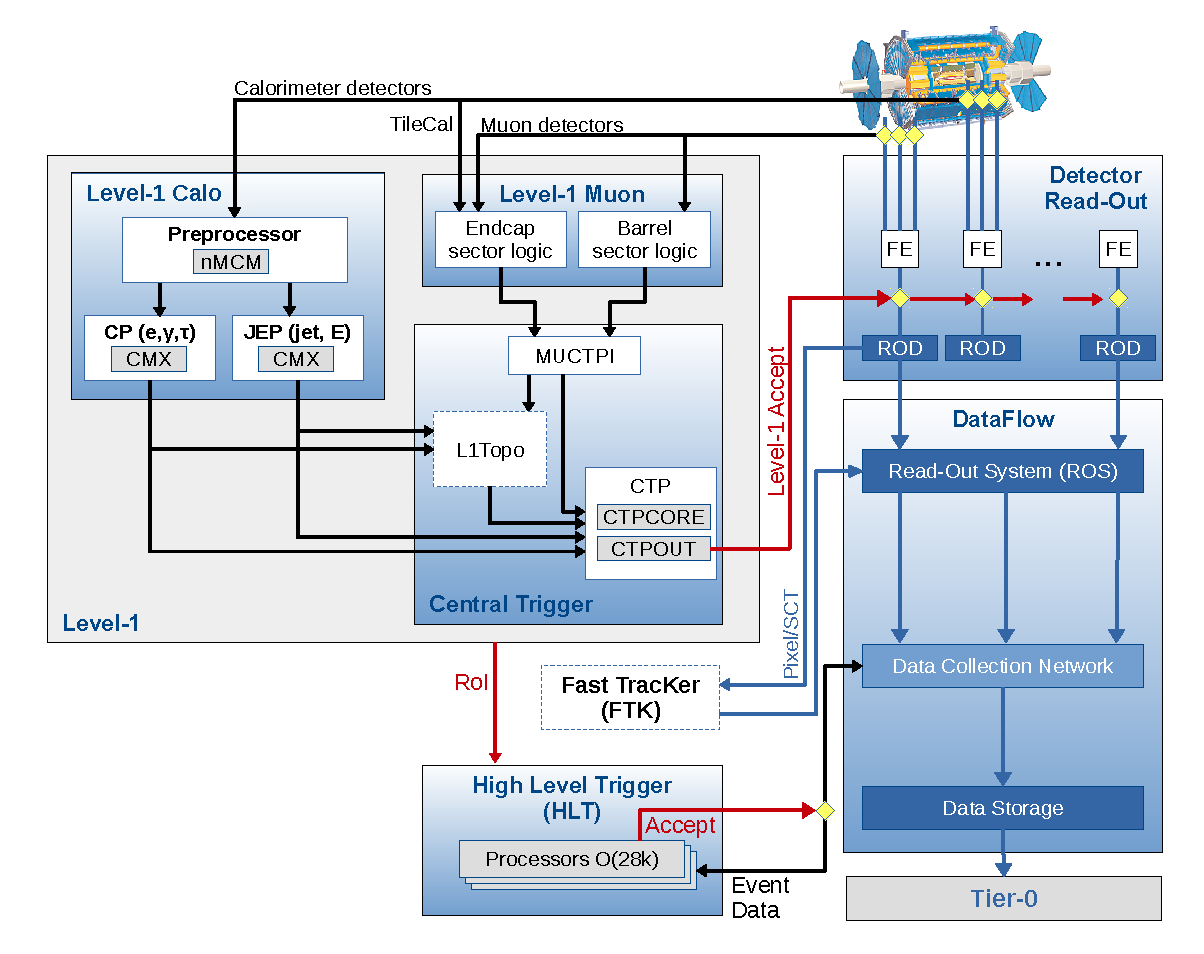
\includegraphics[width=0.9\textwidth]{figures/atlas/tdaq-run2-schematic}}
\caption{Schematic view of the Run 2 \gls{atlas} \gls{tdaq} system. Figure from Ref. \cite{Aaboud:2016leb}.}
\label{fig:atlas:trig}
\end{figure}


\subsection{ATLAS operation}

\gls{atlas} has been successfully recording the collision data delivered by the \gls{lhc} in Run 1 and Run 2. Figure \ref{fig:atlas:lumi1} shows the cumulative luminosity delivered by the \gls{lhc} between the declaration of stable beams and the request to put the detector in standby for beam dump  as well as the luminosity recorded by \gls{atlas} in 2015 and 2016, which is the dataset used in the analyses described in this thesis. The difference between the two derives from inefficiencies of the data acquisition system and from the "warm start" procedure: the high voltage of the tracking devices and the preamplifiers of the pixel detector are turned on after the start of stable beams \cite{LumiTwiki}.

\begin{figure}[ht]
\centering
\subfigure[]{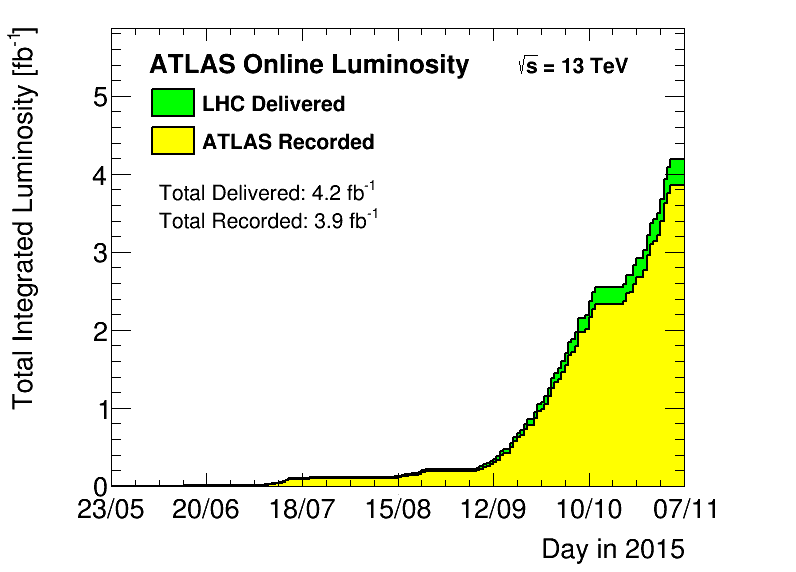
\includegraphics[width=0.48\textwidth]{figures/atlas/lumi/lumi_2015}\label{fig:atlas:lumi1:a}}
\subfigure[]{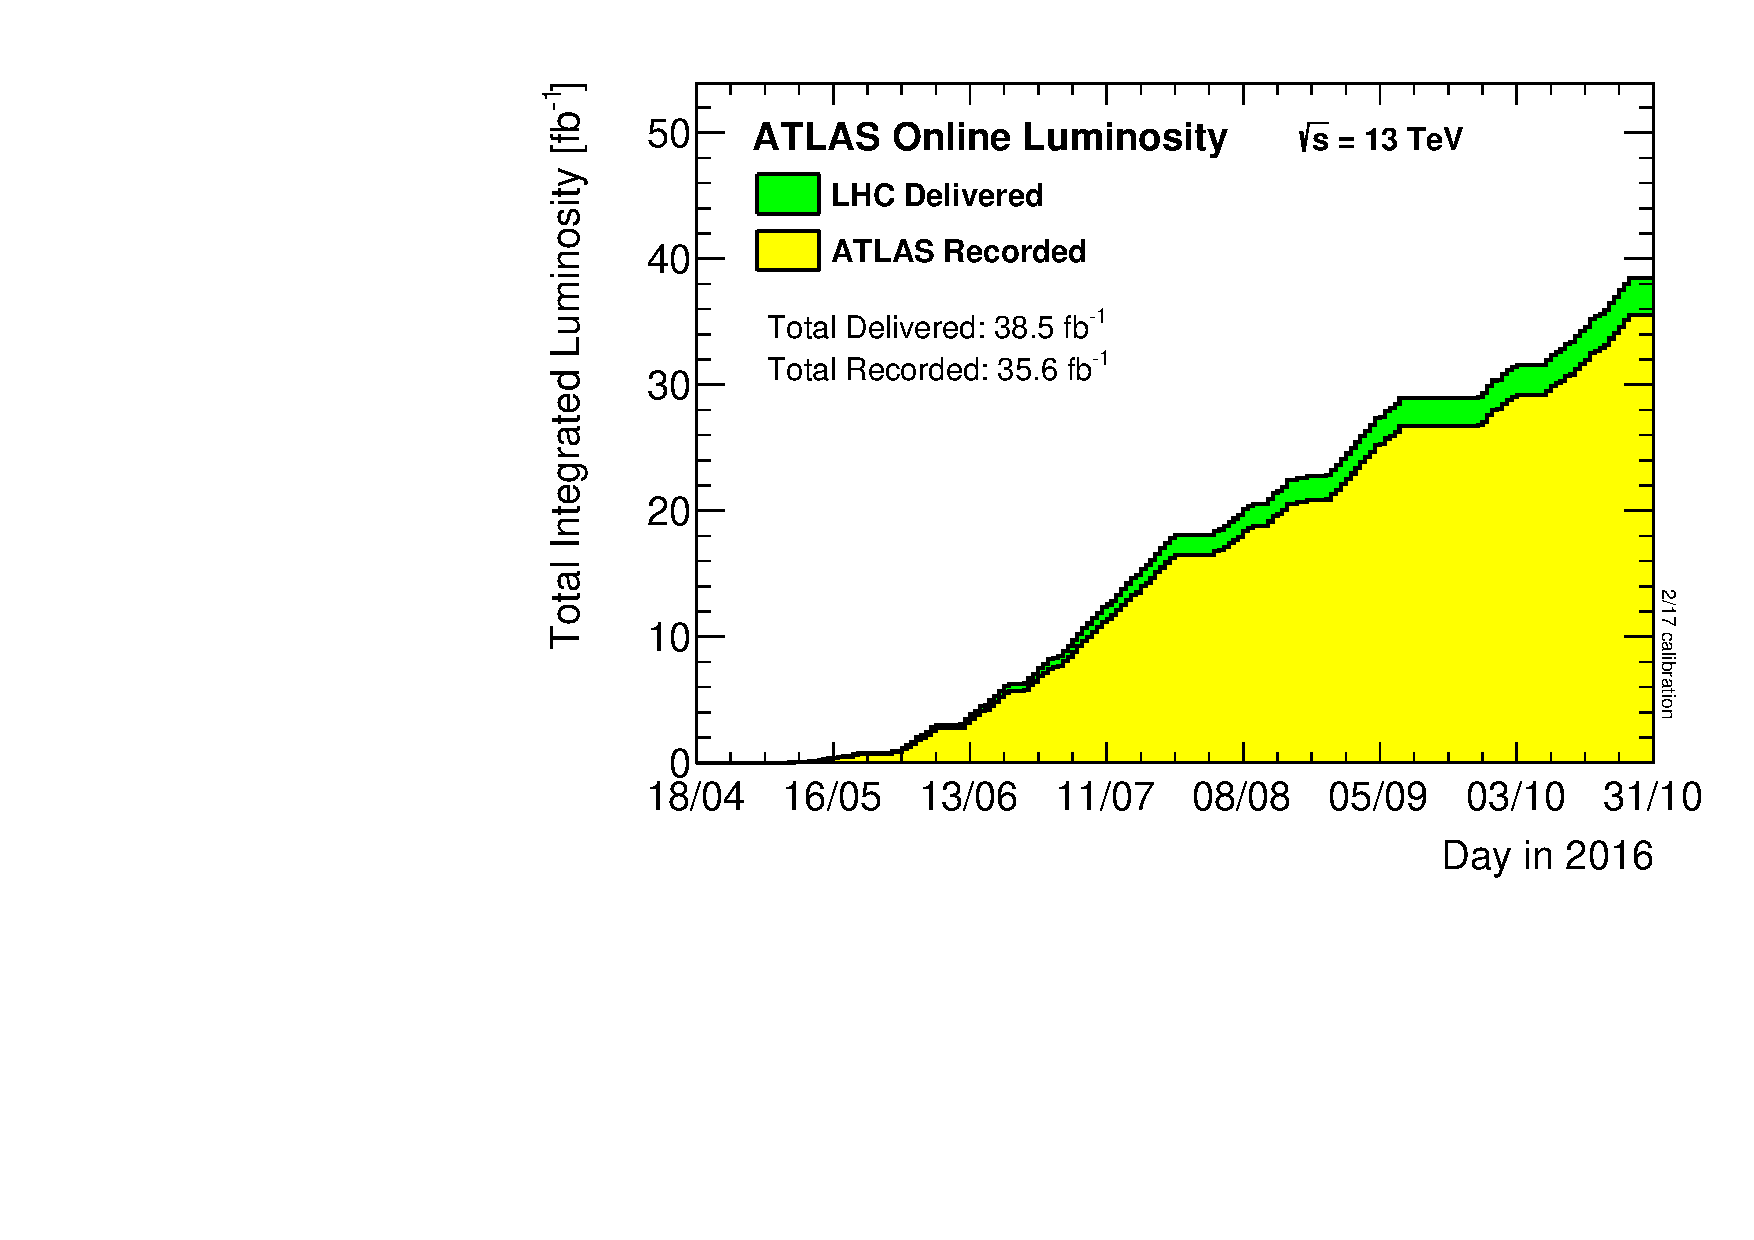
\includegraphics[width=0.48\textwidth]{figures/atlas/lumi/lumi_2016}\label{fig:atlas:lumi1:b}}\\
\subfigure[]{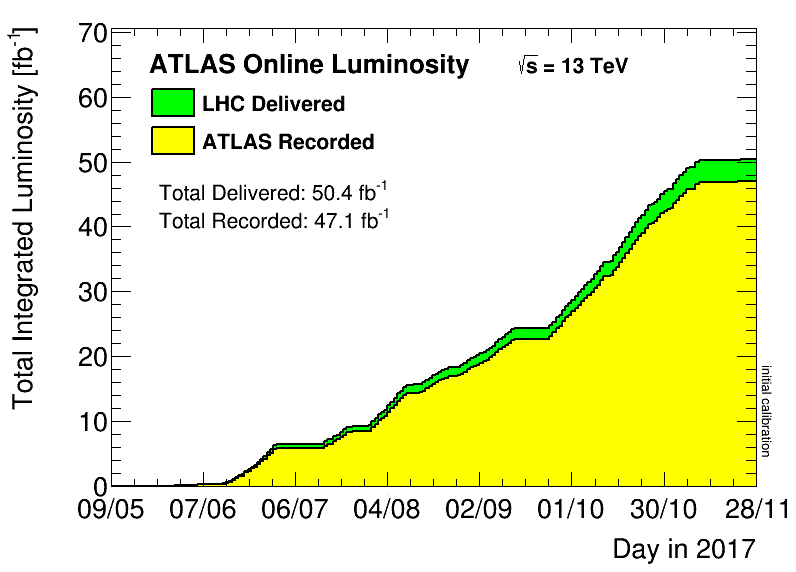
\includegraphics[width=0.48\textwidth]{figures/atlas/lumi/lumi_2017}\label{fig:atlas:lumi1:c}}
\subfigure[]{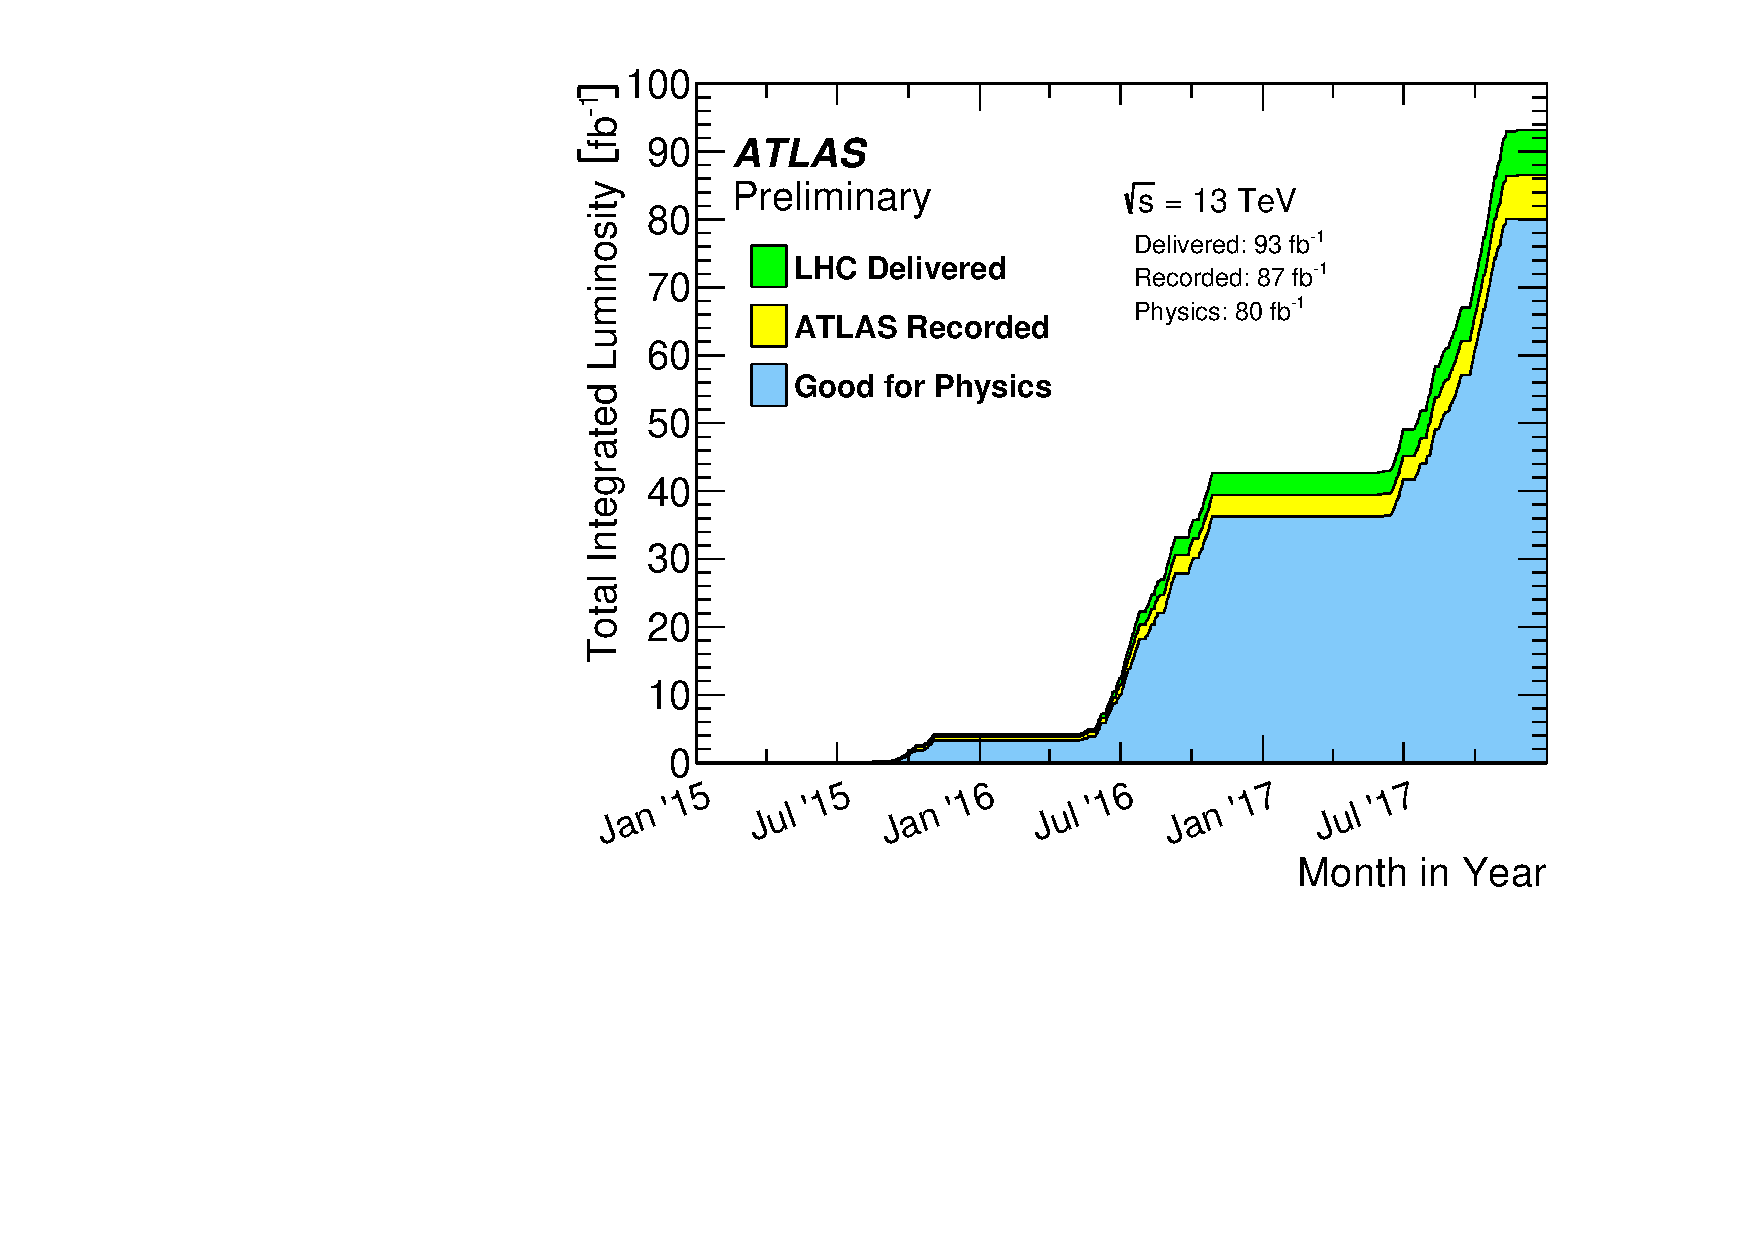
\includegraphics[width=0.48\textwidth]{figures/atlas/lumi/intlumivstimeRun2DQ}\label{fig:atlas:lumi1:d}}
\caption{Cumulative luminosity versus time delivered to (green) and recorded by \gls{atlas} (yellow) during stable beams for pp collisions at $\sqrt{s}=13$ TeV in \subref{fig:atlas:lumi1:a} 2015, \subref{fig:atlas:lumi1:b} 2016, 
and \subref{fig:atlas:lumi1:c} 2017. \subref{fig:atlas:lumi1:d} Cumulative luminosity versus time in 2015-2017 certified to be good quality data (blue). Figure from Ref. \cite{LumiTwiki}.}
\label{fig:atlas:lumi1}
\end{figure}

At the time of this writing, the 2017 dataset has been collected but not yet analyzed. The delivered and recorded luminosity for 2017 is shown in Figure \ref{fig:atlas:lumi1:c}. Not all the recorded luminosity can be used for physics analyses, as most of these require a good state of all the detector subsystems. This is checked for each luminosity block; the ones with poor detector conditions are disregarded, while the ones that pass this criteria form the \gls{grl}, which imposes requirements on the quality of the beams and of the detector. Figure \ref{fig:atlas:lumi1:d} shows the total cumulative luminosity for the 2015-2017 period, highlighting the portion that enters the \gls{grl}. 

